\chapter{Dodatki}
\label{cha:dodatekKLasteryzacja}

\section{k-średnich}
\label{sec:k_means}

\begin{figure}[h]
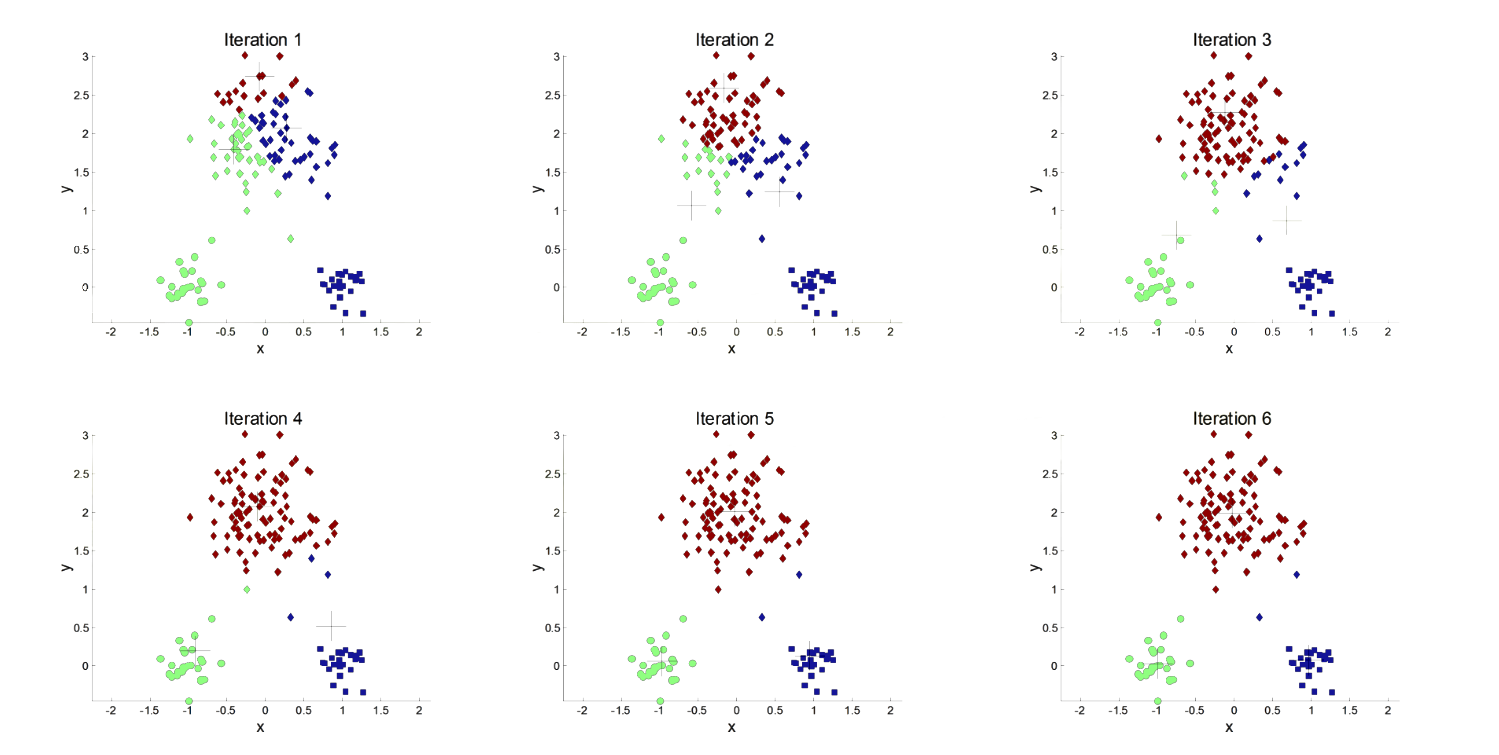
\includegraphics[width=\textwidth]{img/kmeans_startA}
\caption{Warunki początkowe A \cite{Luk}}
\end{figure}

\begin{figure}[H]
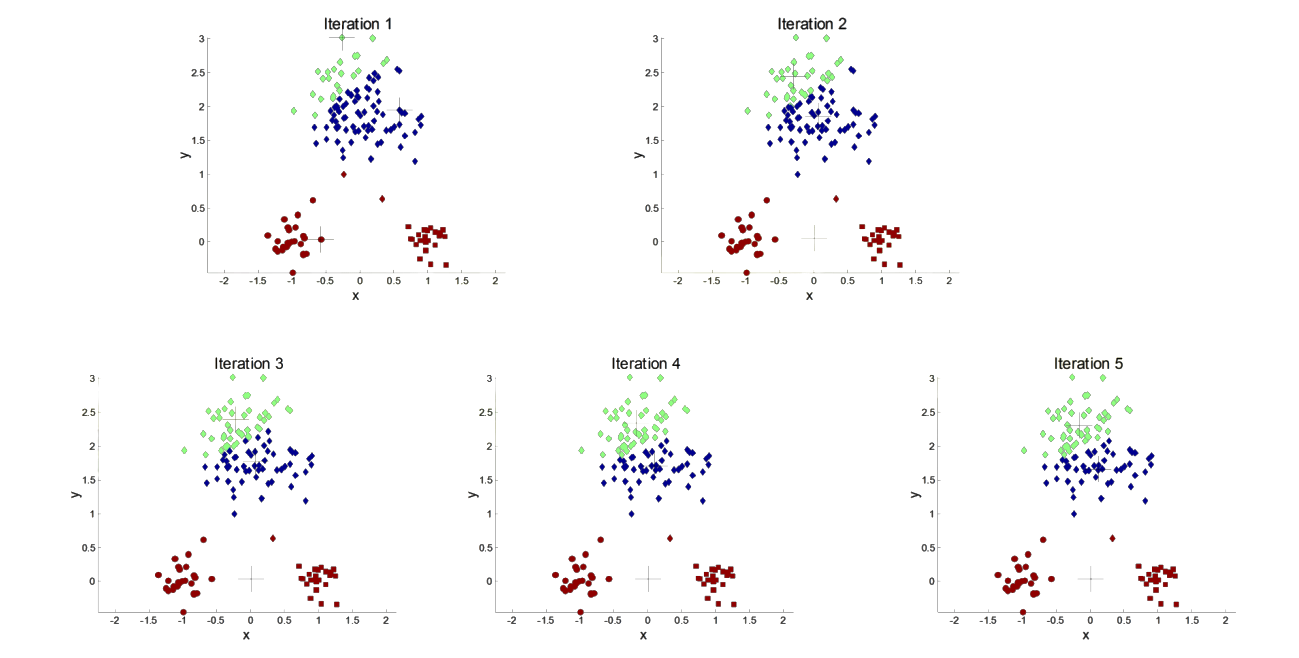
\includegraphics[width=\textwidth]{img/kmeans_startB}
\caption{Warunki początkowe B \cite{Luk}}
\end{figure}

\begin{figure}[H]
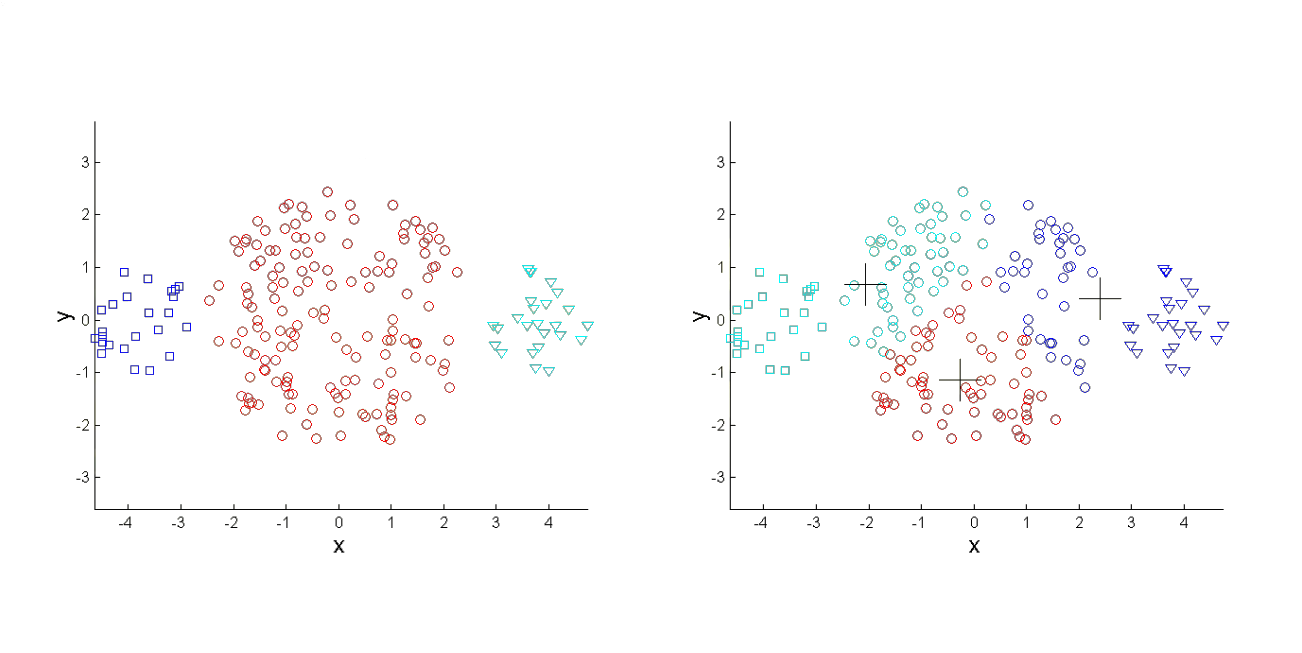
\includegraphics[width=\textwidth]{img/kmeans_quantity}
\caption{Różne liczności klastrów \cite{Luk}}
\end{figure}

\begin{figure}[H]
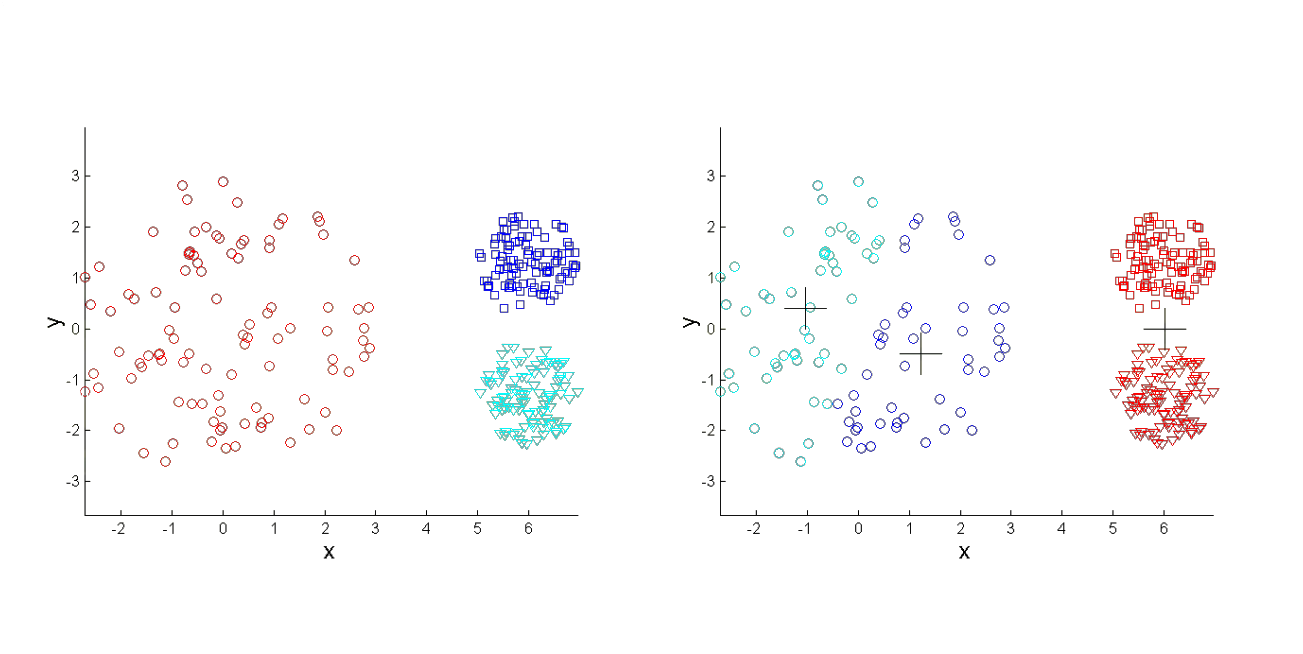
\includegraphics[width=\textwidth]{img/kmeans_density}
\caption{Różne gęstości klastrów \cite{Luk}}
\end{figure}

\begin{figure}[H]
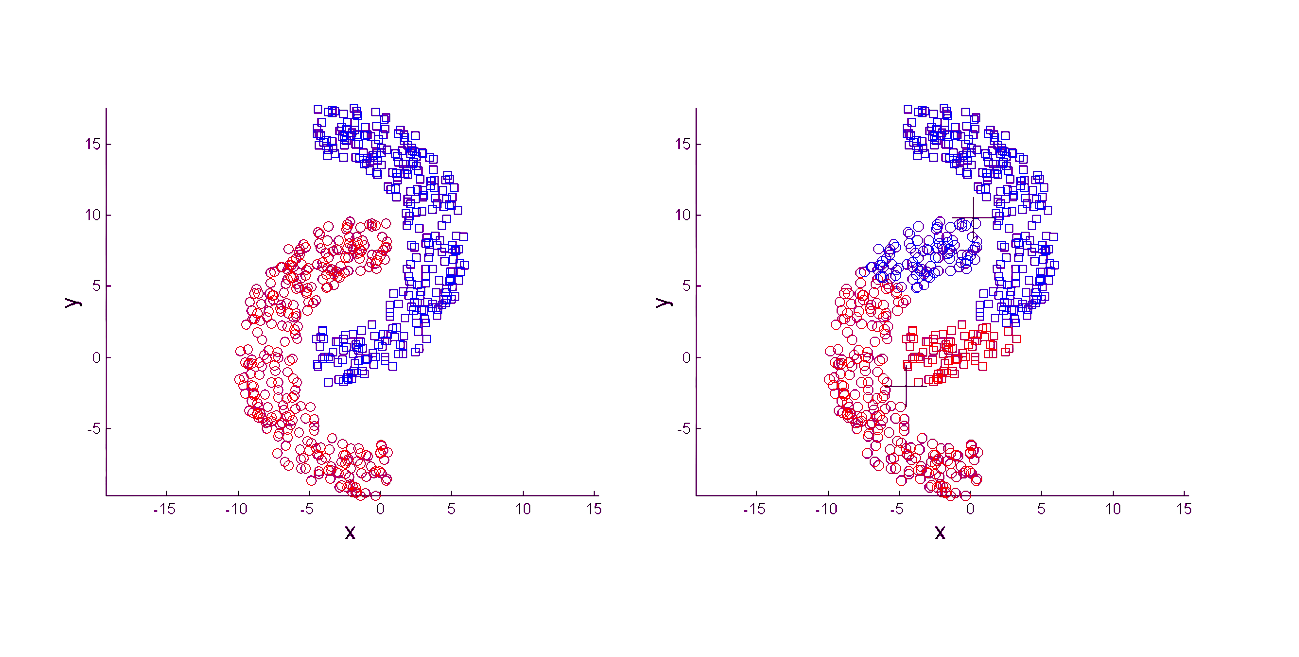
\includegraphics[width=\textwidth]{img/kmeans_irregular}
\caption{Nieregularne kształty klastrów \cite{Luk}} 
\end{figure}

\section{Parametr wygładzania - przykład}
\label{sec:dod_h}

\begin{figure}[H]
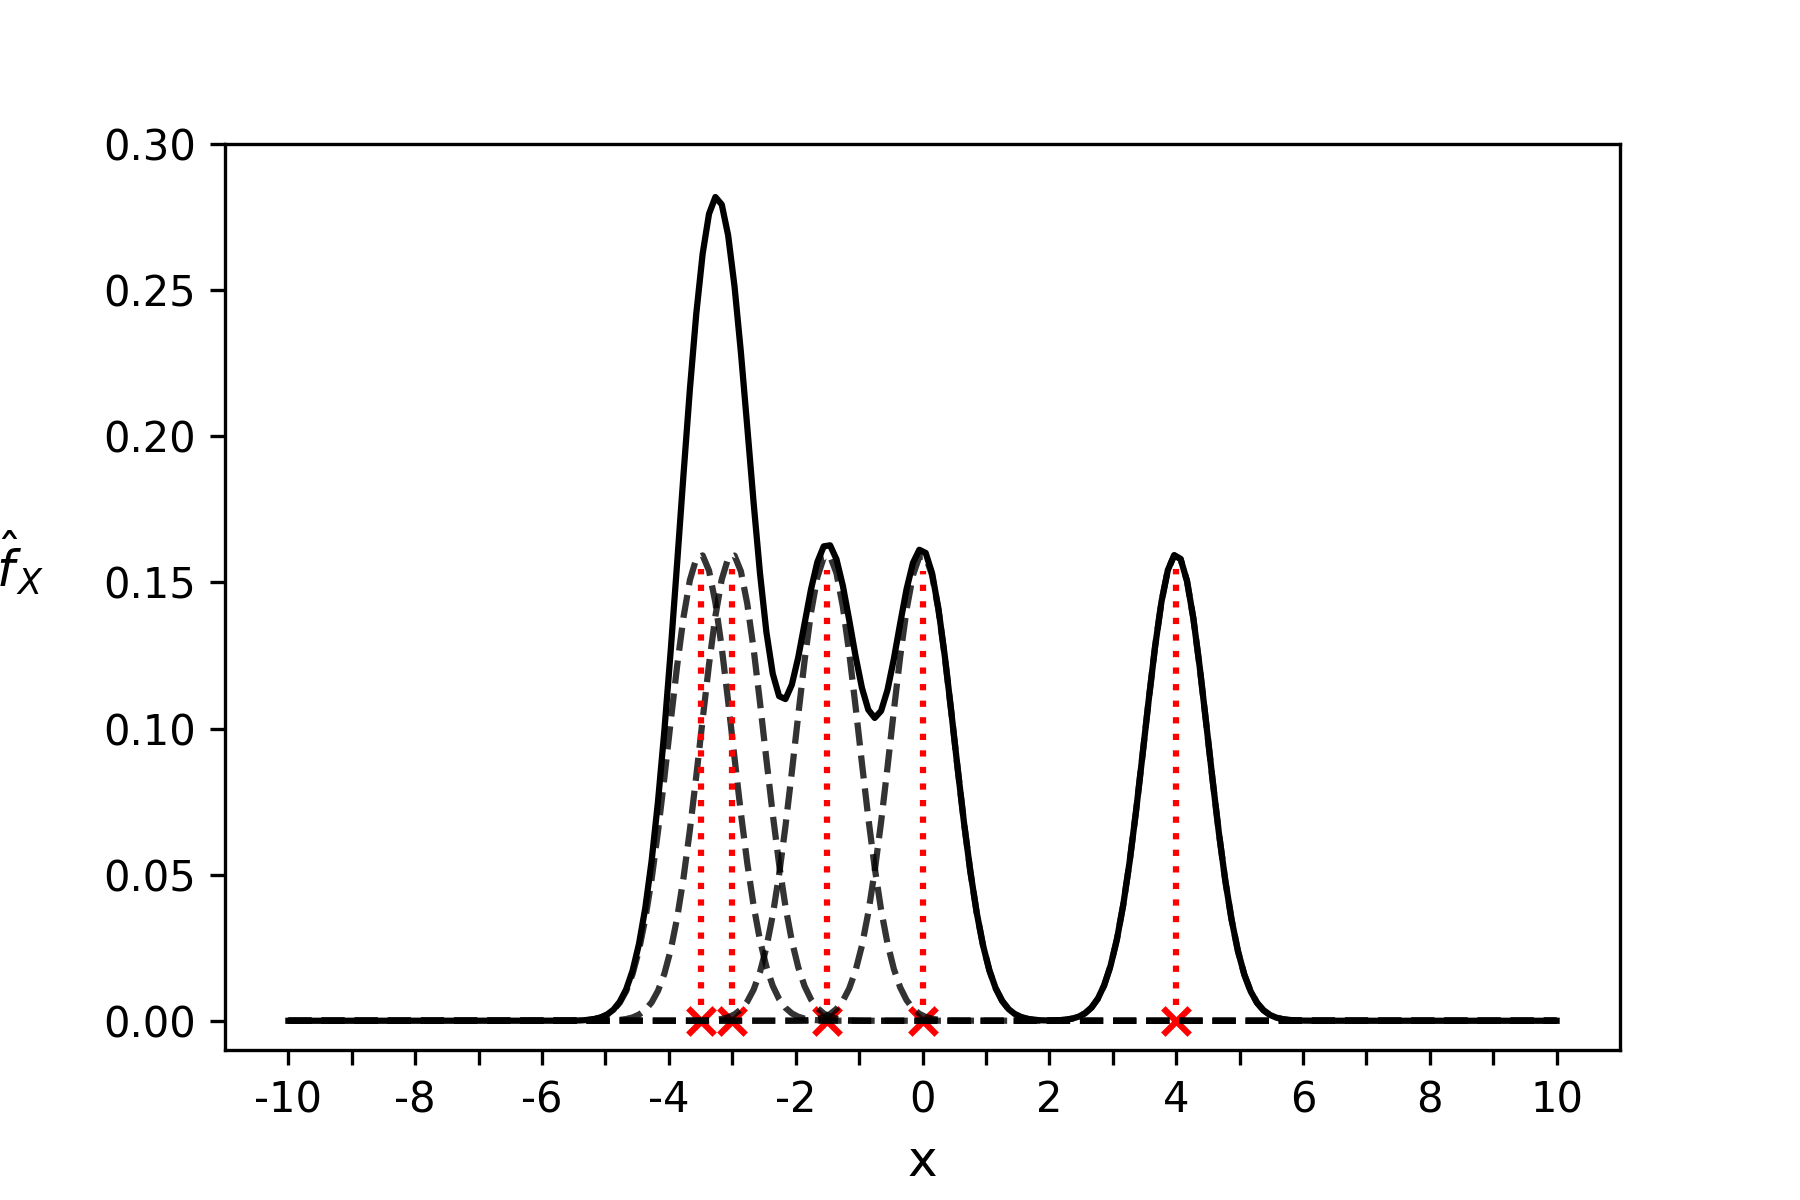
\includegraphics[width=0.9\textwidth]{img/h_05}
\caption{$h=0.5$ \cite{Fra}}
\end{figure}

\begin{figure}[H]
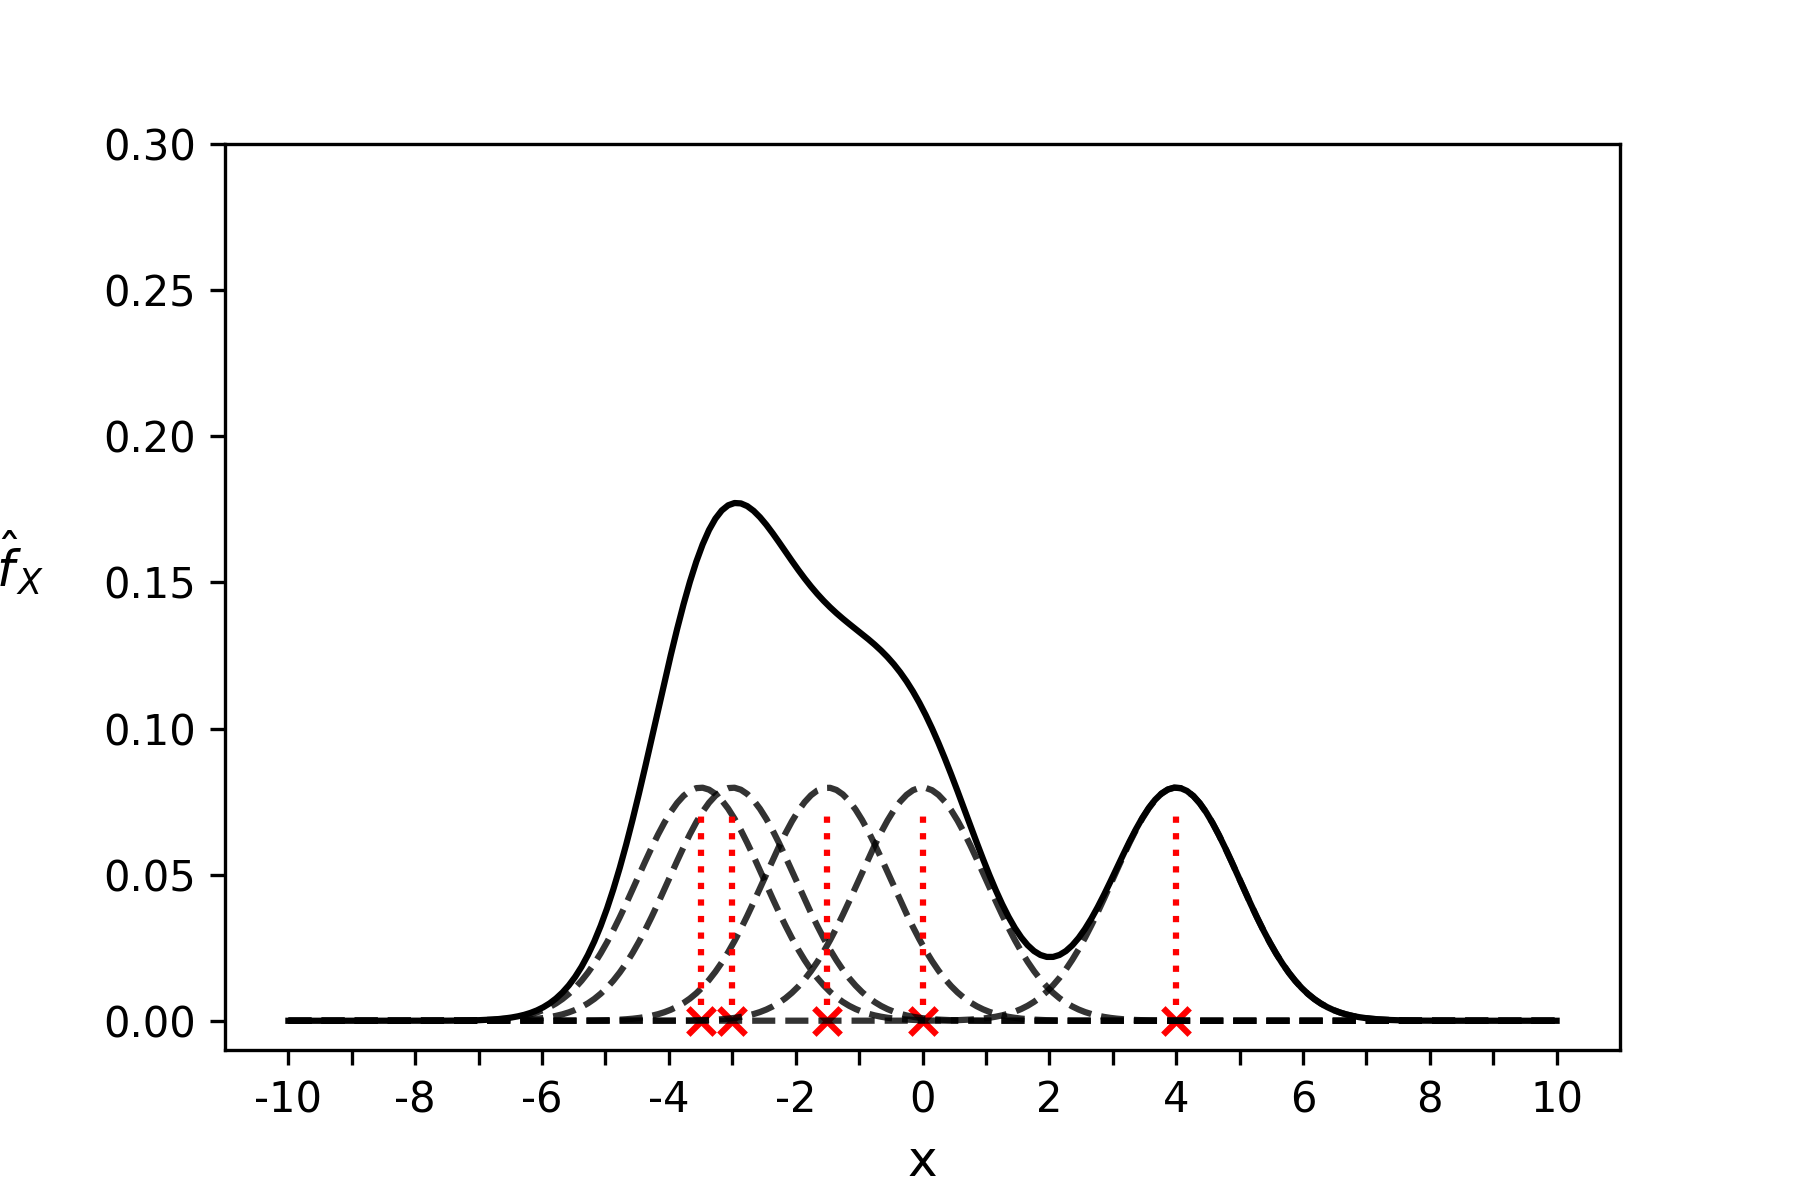
\includegraphics[width=0.9\textwidth]{img/h_1}
\caption{$h=1$ \cite{Fra}}
\end{figure}

\begin{figure}[H]
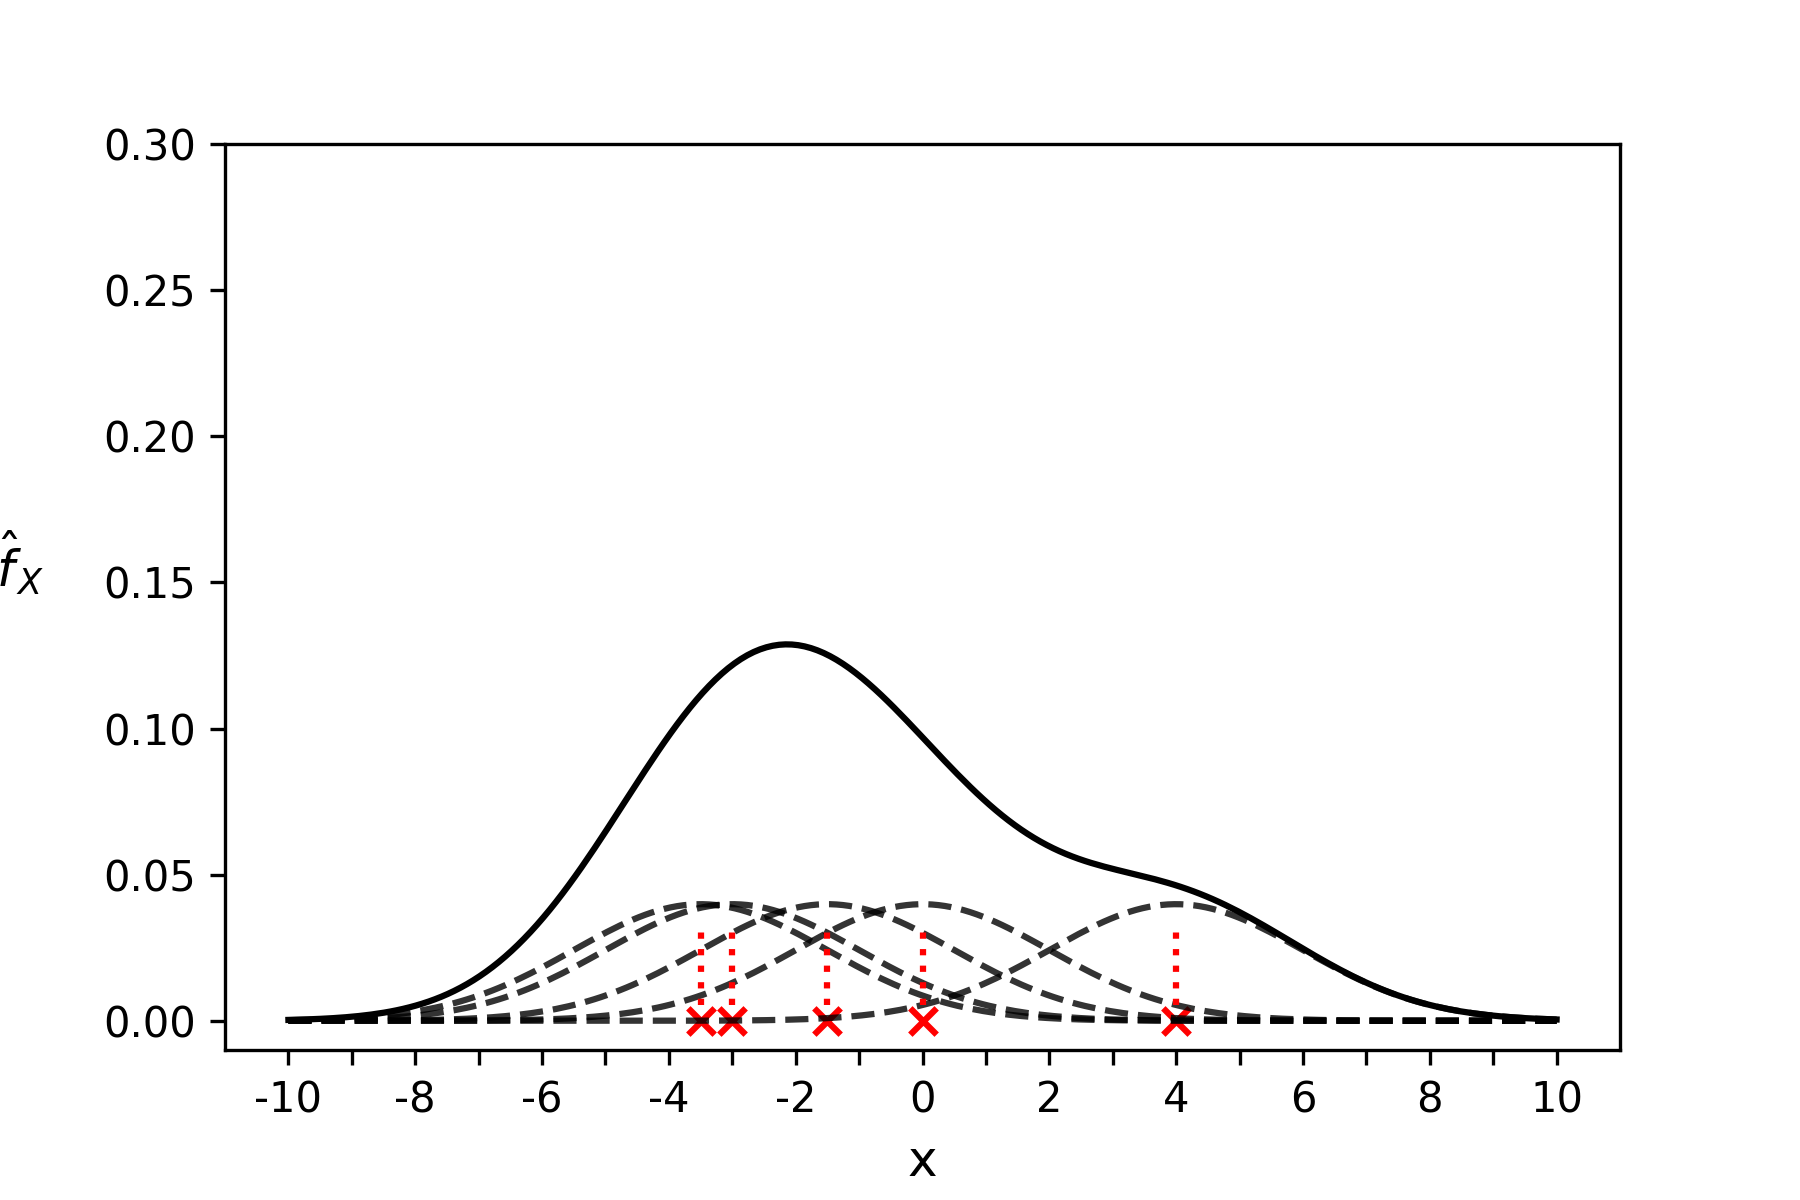
\includegraphics[width=0.9\textwidth]{img/h_2}
\caption{$h=2$ \cite{Fra}}
\end{figure}